% 矩形对角线相等且互相平分
\documentclass[tikz,border=4pt]{standalone}
\usepackage{ctex}
\usepackage{amsmath}
\usetikzlibrary{calc, decorations.markings}
\begin{document}
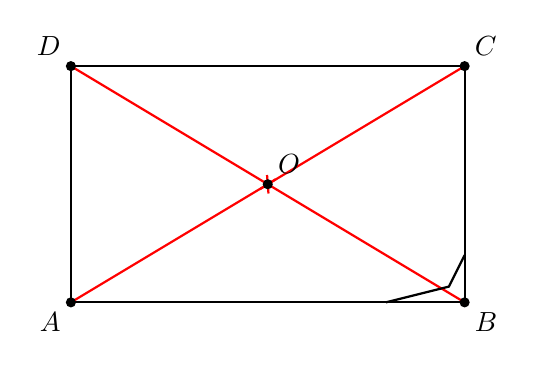
\begin{tikzpicture}[scale=1.0, thick,
  tickone/.style={postaction={decorate, decoration={markings,
    mark=at position 0.5 with {\draw (-1.5pt,-3pt) -- (1.5pt,3pt);}}}},
]
  \coordinate (A) at (0,0);
  \coordinate (B) at (5,0);
  \coordinate (C) at (5,3);
  \coordinate (D) at (0,3);
  \coordinate (O) at ($(A)!0.5!(C)$);
  \draw (A) -- (B) -- (C) -- (D) -- cycle;
  \draw[red, thick, tickone] (A) -- (C);
  \draw[red, thick, tickone] (B) -- (D);
  % 直角标记于 B
  \draw ($(B)!0.2!(A)$) -- ($(B)+(-0.2,0.2)$) -- ($(B)!0.2!(C)$);
  \foreach \pt in {A,B,C,D,O} \filldraw (\pt) circle (1.4pt);
  \node[below left]  at (A) {$A$};
  \node[below right] at (B) {$B$};
  \node[above right] at (C) {$C$};
  \node[above left]  at (D) {$D$};
  \node[above right] at (O) {$O$};
\end{tikzpicture}
\end{document}
